\documentclass[11pt,a4paper]{exam}
\usepackage[utf8x]{inputenc}
\usepackage{ucs}
\usepackage{amsmath}
\usepackage{amsfonts}
\usepackage{amssymb}
\usepackage{graphicx}
\usepackage[left=2.00cm, right=2.00cm, top=2.00cm, bottom=2.00cm]{geometry}
\begin{document}

A = 
$\underset{R}\iint dxdy
=\underset{-2a}{\overset{a}{\mathop \int }}
$$
\left[ \underset{y-a}{\overset{a-\frac{y^2}{a}}{\mathop \int dx}} \right] dy 
=
\underset{-2a}{\overset{a}{\mathop \int }}
\left[|x\underset{y-a}{\overset{a-\frac{y^2}{a}}{\mathop \int}} \right] dy 
= 
\underset{-2a}{\overset{a}{\mathop \int }}
\left[a-\frac{y^2}{a} - ( y - a)  \right] dy 
= 
\underset{-2a}{\overset{a}{\mathop \int }}
\left(2a-\frac{y^2}{a} - y \right) dy 

$
\newpage

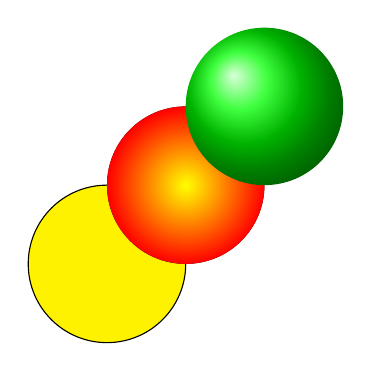
\begin{tikzpicture}
\draw[fill=yellow] (0,0) circle (1);
\fill[inner color=yellow, outer color=red] (1,1) circle (1); \shade[ball color=green] (2,2) circle (1);
\end{tikzpicture}

\end{document}

